\documentclass[12pt]{article}
\setlength\parindent{0pt}
\usepackage{graphicx}
\usepackage[margin=1.0in]{geometry}
\usepackage{amsmath}
\usepackage{ulem}
\usepackage{color}
\usepackage{hyperref}
\setlength{\parindent}{2em}
\graphicspath{ {./images/} }
\title{CTA200H Final Project}
\author{Sarah Thiele}
\date{\today}

\begin{document}
\maketitle

In this project I spent time exploring the usage of COSMIC, or Compact Object and Monte Carlo Investigation Code, a binary population synthesis Python interface. It uses a statistical approach to synthesis, allowing us to create large fixed populations in a relatively short amount of computational time in comparison with normal stellar evolution software. See   \href{https://cosmic-popsynth.github.io/docs/latest/index.html}{\color{blue}\uline{here}} for documentation.

\section{Getting Familiar with COSMIC:}
\subsection{Single binary systems}

I began by installing COSMIC both to my own computer as well as the CITA cluster. This was done by cloing from the public Github repository. As the code is updated often, pulling from git on a semi-regular basis is needed to ensure the most up-to-date processes are in place. 

The next task was to practice with simulating single binary systems. A binary system can be initiated using COSMIC's InitialBinaries method within the InitialBinaryTable class. By trying out various initial parameters (the initial stellar components' masses, their orbital period, eccentricity, and metallicity), I was able to create binaries which when evolved produced double white dwarf (WD), double neutron star (NS), and double black hole (BH) systems. The Evolve package in COSMIC is used for binary evolution, which outputs multiple useful DataFrames. For example, ``bpp" gives parameters at time steps where important changes occur in the system, and ``bcm" gives parameters at the first and final time step. I then found the time step at which the second remnant formed and plotted the evolution of the system's masses, orbital period and eccentricity from Zero Age Main Sequence (ZAMS) until Second Remnant Formation (SRF). This can be done by resetting the time step of the initial conditions table, re-evolving the system with this smaller time step, and extracting the relevant columns until SRF. This data is plotted in Figures 1-4 and the outcome of each system is noted in the respective captions. The initial conditions and final SRF parameters are listed below. Because of the nature of COSMIC's statistical processes we see large and often discontinuous jumps in parameters as the binary system evolves over time. We also see the primary and secondary stars exchange mass when one gains proportional to the others' loss at the same time. This is often accompanied by simultaneous changes in eccentricity and orbital period.

\begin{table}
\centering
\scriptsize
\begin{tabular}{c|cccccccc}
\hline  \\
Remnants &  $m_{1,i}$ $[M_\odot]$ & $m_{2,i}$ $[M_\odot]$ & $e_i$ & P$_{orb,i}$ [days] &  $m_{1,f} $ $[M_\odot]$ & $m_{2,f}$ $[M_\odot]$ & $e_f$ & P$_{orb, f}$ [days] \\
\\
\hline
WD & 4.00 & 6.00 & 0.04 & 40.808 & 0.89 &  1.12 &  0.00 & 0.95 \\
NS  & 16.00 & 15.00 & 0.50 & 400.00 & 1.45 & 1.43 &  0.84 & 1.47\\
BH & 80.00 & 85.00 & 0.01 & 10.05 & 33.58 & 24.91 & 0.01 & 7.27 \\
\hline
\end{tabular}
\label{Table1}
\caption{Summary of the single binary systems' initial conditions and their final parameters at time of SRF.}
\end{table}


\begin{figure}
    \centering
    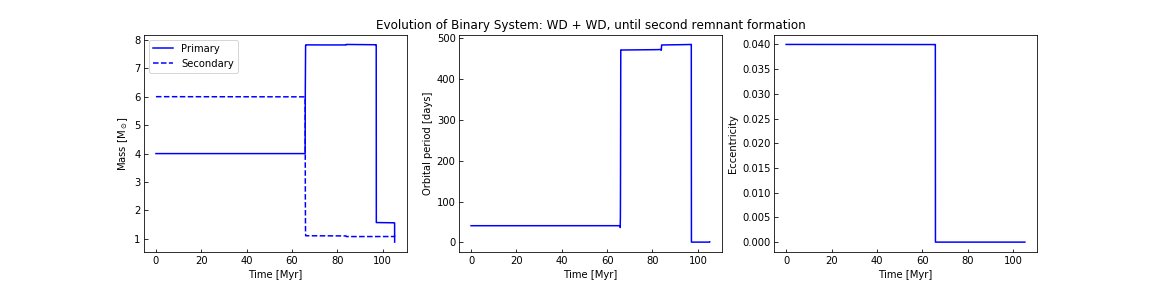
\includegraphics[trim={4cm 0 4cm 0},clip, 
    scale=0.45]{WD_bin_3panel.png}
    \caption{A system which forms a WD + WD binary system. The system survives undisrupted for the full 13.7 Gyr evolution.}
    \label{Figure1}
\end{figure}

\begin{figure}
    \centering
    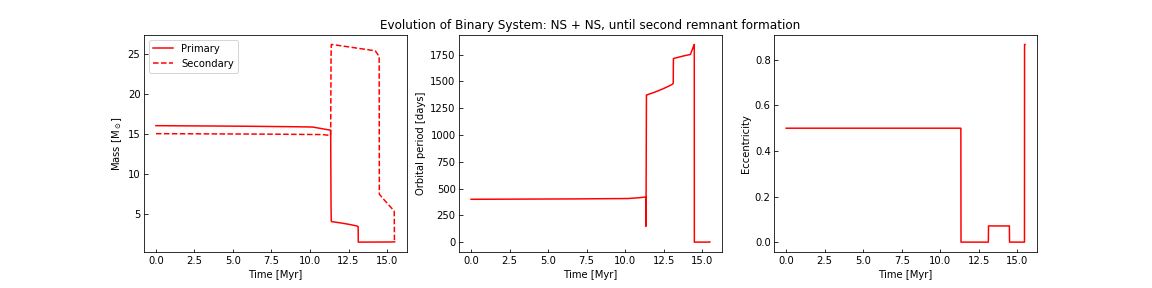
\includegraphics[trim={3cm 0 4cm 0},clip, 
    scale=0.45]{NS_bin_3panel.png}
    \caption{A system which forms a NS + NS binary system. The system eventually merges into a single black hole.}
    \label{Figure2}
\end{figure}
\begin{figure}
    \centering
    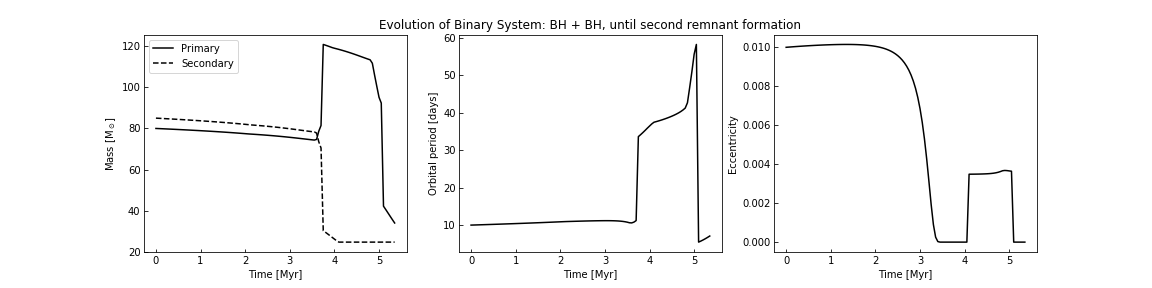
\includegraphics[trim={3.5cm 0cm 4cm 0},clip, 
    scale=0.45]{BH_bin_3panel.png}
    \caption{A system which forms a BH + BH binary system.  The binary survives undisrupted for the full 13.7 Gyr evolution.}
    \label{Figure3}
\end{figure}
\begin{figure}
    \centering
    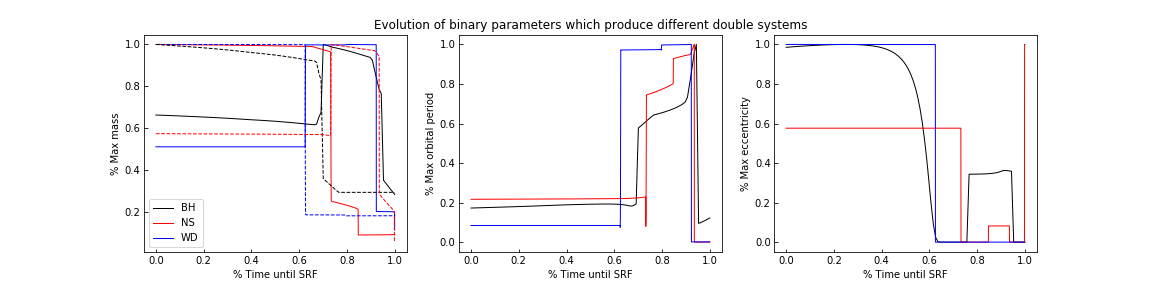
\includegraphics[trim={3.5cm 1cm 4cm 0},clip, 
    scale=0.45]{All_3panel.png}
    \caption{All binary systems evolution plotted as percentages of the maximum of the respective parameters. All three systems undergo mass transfer and large temporary jumps in orbital period before converging to their final states.}
    \label{Figure4}
\end{figure}

\pagebreak
\subsection{Binary grid}

Here a grid of initial binaries was run to see how changing the secondary mass impacts the outcome of the system. I used primary masses from $10$ to 100 M$_\odot$, and for each primary mass a grid was created with 10 secondary masses with a mass ratio $m_2 / m_1$ ranging from 0.1 to 1.0. The initial orbital periods were 50 days, with eccentricities of 0.5. I then selected the orbital period for each ($m_1, m_2$) combination at the time of SRF. These were then plotted as a function of mass ratio for each primary mass. These plots are shown in Figure 5 and 6. 

An orbital period of 0.0 indicates a merging event, a supernova of one/both of the stars, or an outcome from a common envelope phase, resulting in a massless remnant(s) as the system's outcome. An orbital period of -1.0 indicates a disrupted system, which is more likely the further the separation between bodies is. We see in \autoref{Figure5} that when the other initial conditions are held constant, binaries with a smaller total mass had much higher merger/disruption fraction for these conditions compared with the higher mass systems. For example, for a 10 M$_\odot$ primary mass, none of the binary systems survive, but 70\% of the systems with a primary mass of 100 M$_\odot$ survive, creating double BH binaries.

In \autoref{Figure6}, all of the data is plotted together. There is no data above an orbital period of 20 days for primary masses greater than 50 M$_\odot$, with lower primary masses sitting mainly below 10 days, with most below 40 M$_\odot$ disrupted/merged.


\begin{figure}
    \centering
    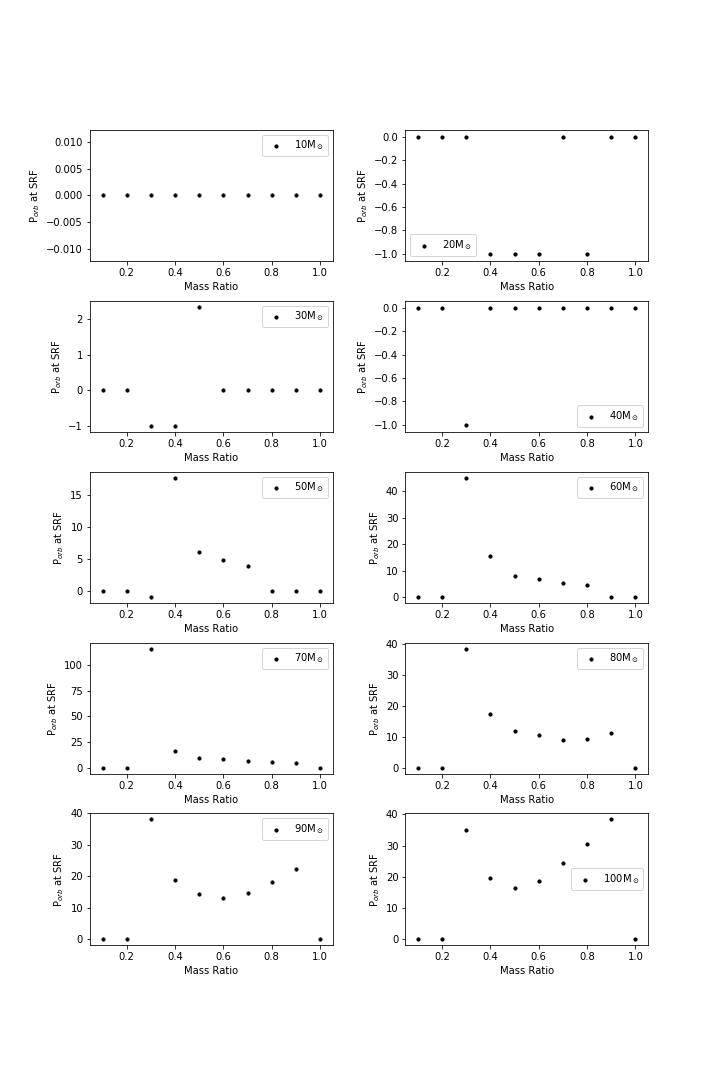
\includegraphics[trim={1cm 2cm 1cm 2cm},clip, 
    scale=0.6]{Period_Grid_Panels.png}
    \caption{Orbital period at SRF for various primary and secondary masses, with an initial orbital period of 50 days and eccentricity of 0.5. Legend indicates the primary mass.}
    \label{Figure5}
\end{figure}

\begin{figure}
    \centering
    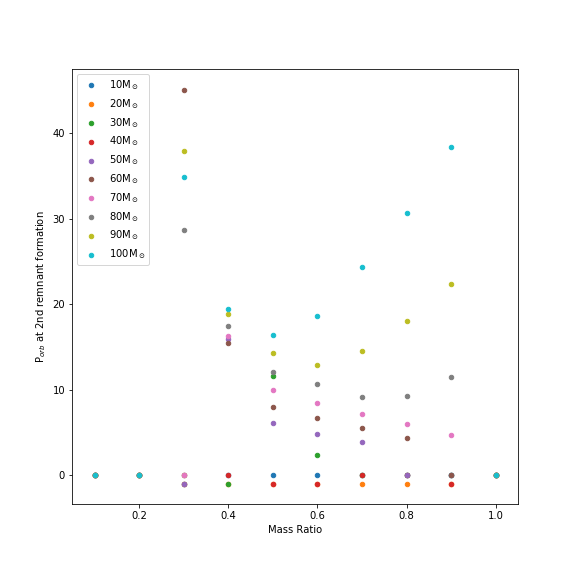
\includegraphics[trim={1cm 0 1cm 1cm},clip, 
    scale=0.8]{Period_Grid_All.png}
    \caption{Orbital period at SRF for various primary and secondary masses, with an initial orbital period of 50 days and eccentricity of 0.5. P$_{orb}$ is in days. The legend indicates the primary mass.}
    \label{Figure6}
\end{figure}

\section{Simulating double white dwarf populations}
\subsection{Methods}

Our next goal was to simulate two double white dwarf populations with changes to a single parameter for comparison. We can use COSMIC's independent sampler to generate a binary population by hand. Within the independent sampler, one can input the desired final stellar type, and choose independent models for each parameter. For example, in this setup we used a model for eccentricity following a uniform distribution, and with metallicity Z=0.017. We initialize the binaries with a star formation burst 13.7 Gyr in the past. These binaries can then be evolved in the same way as before using the Evolve package in COSMIC. 

Due to issues with working with the CITA cluster we were unable to initialize the original goal of 1,000,000 binaries; a segmentation fault occured for higher than 1,000, so we lowered our population size to this instead. These binaries were initialized separately from the jupyter notebook for this project, coded on the CITA cluster ``bubbles" under the scripts sim.py and sim\_2.py, which will be attached in the Github repository for this project.

Next, from the output systems, all the WD + WD binaries were selected by masking over the stellar type column for WD types: either Carbon/Oxygen, Oxygen/Neon, or Helium WDs. We can find the age of the binary as the time from ZAMS to SRF, as well as the systems' masses and orbital periods at SRF. These are plotted in histograms in \autoref{Figure7}. 

We can also study the time it would take each binary to merge from the time of SRF. This can be found by solving differential equations for the change in semi-major axis and eccentricity with respect to time. From \href{https://ui.adsabs.harvard.edu/abs/1964PhRv..136.1224P/abstract}{\color{blue}\uline{Peters (1964)}}, we have:
\begin{align}
    \frac{da}{dt} &= -\frac{64}{5}\frac{G^3m_1m_2(m_1+m_2)}{c^5a^3(1-e^2)^{7/2}}\left(1+\frac{73}{24}e^2+\frac{37}{96}e^4\right) \label{Eq1} \\
    \frac{de}{dt} &= -\frac{304}{15}e\frac{G^3m_1m_2(m_1+m_2)}{c^5a^4(1-e^2)^{5/2}}\left(1+\frac{121}{304}e^2\right)
\end{align}


The mass values are those at the time of SRF, and $a_0$ is the separation of the two WDs at SRF. We expect that all the WD + WD binaries to be in approximately circular obits. For circular binaries ($e=0.0$), \autoref{Eq1} can be solved for the semi-major axis as a function of time, and can be simplified by defining a constant $\beta$ (\autoref{Eq3}). We can then define the time it takes for the binary to merge $T_m$ by setting $a(t)=0.0$:
\begin{align}
    \beta &= \frac{64}{5}\frac{G^3m_1m_2(m_1+m_2)}{c^5} \label{Eq3}\\
    a(t) &= (a_0^4 - 4\beta t)^{1/4} \label{Eq.2} \\
    T_m(a_0) &= \frac{a_0^4}{4\beta}
\end{align}

The delay time, defined as the time it would take for a binary system to merge from its ZAMS system formation, is then simply the sum of the age of each binary system at SRF time and the merger time:
$$T_{delay} = T_{ZAMS} + T_m $$

Within a dictionary of flags/parameters which are fed into the binary evolution models with COSMIC, denoted BSEDict, there is a parameter alpha which describes the common-envelope efficiency. It dictates the efficiency with which orbital energy is transferred to the envelope surrounding a binary system. A common envelope is when the binary system is contained completely within a gas, sometimes arising from unstable mass transfer. The gas doesn't necessarily rotate at the same rate as the binary system, and so the common envelope phase is thought to bring binary systems to closer separations due to this energy and momentum transfer, often causing a merger if it is not expelled in a short enough period of time while the stars inspiral. For the first set of initializations, alpha=1.0 (\autoref{Figure7}). This was then redone with alpha=0.25 (\autoref{Figure8}). The delay time is plotted as a log plot as this was more informative than a regular histogram.
\begin{figure}
    \centering
    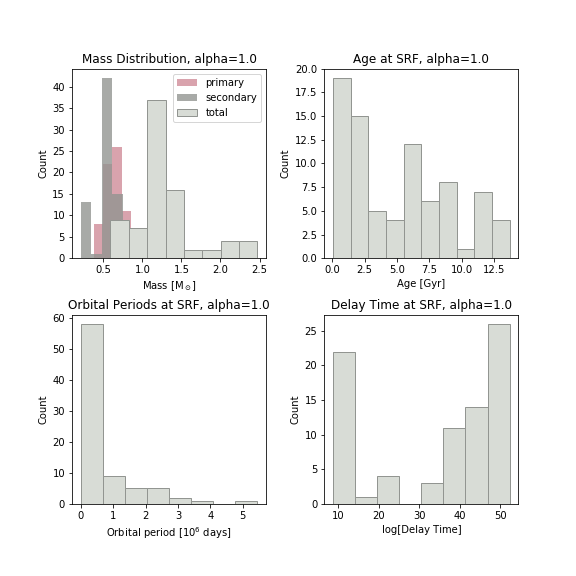
\includegraphics[trim={1cm 1cm 2cm 1cm},clip, scale=0.5]{WDBins_a1.png}
    \caption{Parameter distributions of population of WD + WD binaries, common envelope efficiency alpha=1.0.}
    \label{Figure7}
\end{figure}
\begin{figure}
    \centering
    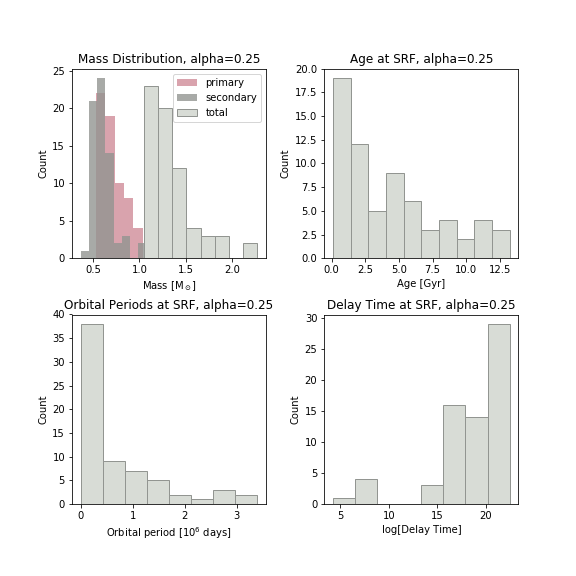
\includegraphics[trim={1cm 1cm 2cm 1cm}, clip, scale=0.5]{WDBins_a025.png}
    \caption{Parameter distributions of population of WD + WD binaries, common envelope efficiency alpha=0.25.}
    \label{Figure8}
\end{figure} 

\pagebreak
\subsection{Comparison between alpha=1.0 and alpha=0.25 populations}
From the initialized populations of $\sim$1000, only 81 become WD + WD binaries from the alpha=1.0 population, and 67 from the alpha=0.25 population. In both cases, the masses of the WDs are generally between 0.5 and 1.0 M$_\odot$ as expected. However, for alpha=0.25, all of the total system masses are greater than 1.0 M$_\odot$, whereas for alpha=1.0 there is closer to a normal distribution of mass. Both systems have a peak total mass between 1.0-1.25 M$_\odot$. The age of SRF has a distribution skewed slightly more to younger ages for alpha=0.25 than for alpha=1.0. The orbital periods for alpha=0.25 have a few more stars at higher orbital periods (past the leftmost histogram bin) and thus larger separations than for alpha=1.0. This is consistent with our earlier discussion of the effects of common envelope efficiency. When there is a lower efficiency of orbital energy and momentum transfer, the closing of separation of the binary system will not occur as effectively and thus we are left with more long-range binary systems as a result. The largest effect of changing the alpha parameter is in the delay times. $\log[T_{delay}]$ produces a large population between 10-15 for alpha=1.0, which is completely missing from the alpha=0.25 population. This can again be related to the efficiency of the common envelope phase. Binaries which go through a more effective common envelope phase will be brought closer together on shorter timescales are are more likely to merge.

\end{document}